\documentclass{beamer}[10]

\usepackage{graphicx}
\usepackage{xcolor}
\usepackage{tabto}
%\usepackage{beamerthemesplit}
\usepackage{tikz}
\usepackage{cancel}
\usepackage{verbatim}
\usepackage{fancybox}
\usepackage{enumerate}
\usepackage{amsmath,amssymb,amsthm,textcomp,mathtools}
\usepackage[super]{nth}
\usepackage[amssymb]{SIunits}
\usepackage{booktabs}
\usepackage{cancel}
\usepackage{bm}
\usepackage[utf8]{inputenc}
\usepackage{tabularx}
\usepackage{ragged2e}
\newcolumntype{Y}{ >{\RaggedRight\arraybackslash}X}
\usetikzlibrary{arrows,shapes}
\newcommand\T{\rule{0pt}{2.6ex}}
\newcommand\B{\rule[-1.2ex]{0pt}{0pt}}
\definecolor{UUcrimson}{RGB}{204,0,0}
\mode<presentation>
{ \usetheme{default}
  \usecolortheme[named=UUcrimson]{structure}
  \useinnertheme{circles}
  \setbeamercovered{transparent}
  \setbeamertemplate{blocks}[rounded]
  \usefonttheme[onlymath]{serif}
  \setbeamertemplate{navigation symbols}{}
  \setbeamertemplate{footline}[page number]
  \setbeamertemplate{navigation symbols}{}
  \setbeamercolor{section in toc}{fg=black,bg=white}
  \setbeamercolor{alerted text}{fg=UUcrimson!80!gray}
  \setbeamercolor*{palette primary}{fg=white,bg=UUcrimson}
  \setbeamercolor*{palette secondary}{fg=UUcrimson!70!black,bg=gray!15!white}
  \setbeamercolor*{palette tertiary}{bg=UUcrimson!80!black,fg=gray!10!white}
  \setbeamercolor*{palette quaternary}{fg=UUcrimson,bg=gray!5!white}
  \setbeamercolor*{palette sidebar primary}{fg=UUcrimson!10!black}
  \setbeamercolor*{palette sidebar secondary}{fg=white}
  \setbeamercolor*{palette sidebar tertiary}{fg=UUcrimson!50!black}
  \setbeamercolor*{palette sidebar quaternary}{fg=gray!10!white}
  \setbeamercolor{titlelike}{parent=palette primary,fg=white}
  \setbeamercolor{frametitle}{bg=UUcrimson}
  \setbeamercolor{frametitle right}{bg=UUcrimson}
  \setbeamercolor*{separation line}{}
  \setbeamercolor*{fine separation line}{}
}

\usetikzlibrary{backgrounds}
\makeatletter
\tikzstyle{every picture}+=[remember picture]
\tikzset{%
  fancy quotes/.style={
    text width=\fq@width pt,
    align=justify,
    inner sep=1em,
    anchor=north west,
    minimum width=\linewidth,
    font=\itshape
  },
  fancy quotes width/.initial={.8\linewidth},
  fancy quotes marks/.style={
    scale=8,
    text=white,
    inner sep=0pt,
  },
  fancy quotes opening/.style={
    fancy quotes marks,
  },
  fancy quotes closing/.style={
    fancy quotes marks,
  },
  fancy quotes background/.style={
    show background rectangle,
    inner frame xsep=0pt,
    background rectangle/.style={
      fill=gray!25,
      rounded corners,
    },
  }
}
\newenvironment{fancyquotes}[1][]{%
\noindent
\tikzpicture[fancy quotes background]
\node[fancy quotes opening,anchor=north west] (fq@ul) at (0,0) {``};
\tikz@scan@one@point\pgfutil@firstofone(fq@ul.east)
\pgfmathsetmacro{\fq@width}{\linewidth - 2*\pgf@x}
\node[fancy quotes,#1] (fq@txt) at (fq@ul.north west) \bgroup}
{\egroup;
\node[overlay,fancy quotes closing,anchor=east] at (fq@txt.south east) {''};
\endtikzpicture}
\makeatother


\usetikzlibrary{backgrounds}
\makeatletter
\tikzstyle{every picture}+=[remember picture]
\tikzset{%
  fancy defs/.style={
    text width=\fq@width pt,
    align=justify,
    inner sep=0.25em,
    anchor=north west,
    minimum width=\linewidth,
    font=\itshape
  },
  fancy defs width/.initial={.8\linewidth},
  fancy defs marks/.style={
    scale=8,
    text=white,
    inner sep=0pt,
  },
  fancy defs opening/.style={
    fancy defs marks,
  },
  fancy defs closing/.style={
    fancy defs marks,
  },
  fancy defs background/.style={
    show background rectangle,
    inner frame xsep=0pt,
    background rectangle/.style={
      fill=gray!25,
      rounded corners,
    },
  }
}
\newenvironment{fancydefs}[1][]{%
\noindent
\tikzpicture[fancy defs background]
\node[fancy defs opening,anchor=north west] (fq@ul) at (0,0) {};
\tikz@scan@one@point\pgfutil@firstofone(fq@ul.east)
\pgfmathsetmacro{\fq@width}{\linewidth - 2*\pgf@x}
\node[fancy defs,#1] (fq@txt) at (fq@ul.north west) \bgroup}
{\egroup;
\node[overlay,fancy defs closing,anchor=east] at (fq@txt.south east) {};
\endtikzpicture}
\makeatother
\usepackage{scalerel}[2014/03/10]
\usepackage{stackengine}
\usepackage{empheq}
\newcommand*\widefbox[1]{\fbox{\hspace{0.5em}#1\hspace{0.5em}}}

\newcommand\reallywidetilde[1]{\ThisStyle{%
  \setbox0=\hbox{$\SavedStyle#1$}%
  \stackengine{-.1\LMpt}{$\SavedStyle#1$}{%
    \stretchto{\scaleto{\SavedStyle\mkern.2mu\sim}{.5467\wd0}}{.4\ht0}%
%    .2mu is the kern imbalance when clipping white space
%    .5467++++ is \ht/[kerned \wd] aspect ratio for \sim glyph
  }{O}{c}{F}{T}{S}%
}}
\usepackage{media9}

\logo{
\includegraphics[width=0.75cm]{logo.jpg}}
\author[Gibbs]{Dr. Jeremy A. Gibbs}
\institute{Department of Mechanical Engineering\\University of Utah}
\date{Spring 2017}
\title{Environmental Fluid Dynamics: Lecture 24}
% colors
\newcommand{\ihat}{\boldsymbol{\hat{\imath}}}
\newcommand{\jhat}{\boldsymbol{\hat{\jmath}}}
\newcommand{\khat}{\boldsymbol{\hat{k}}}
\definecolor{colororange}{HTML}{E65100} % orange
\definecolor{colordgray}{HTML}{795548} % dark gray for note
\definecolor{colorhgray}{HTML}{212121} % heavy dark gray for normal text
\definecolor{colorgreen}{HTML}{009688} % green
\definecolor{colorwhite}{HTML}{FFFFFF} % background white
\definecolor{colorlgray}{HTML}{F5F3EE} % background light gray
\definecolor{colorblue}{HTML}{0277BB} % blue
\definecolor{colorred}{HTML}{CC0000} % red
\newcommand{\fontsizeone}{1.9em}
\setbeamertemplate{caption}{\raggedright\insertcaption\par}
\newcommand{\framecard}[2][colorgreen]{
  {\setbeamercolor{background canvas}{bg=#1}
    \begin{frame}[plain]
    \vfill
    \begin{center}
     {#2}
    \end{center}
    \vfill
    \end{frame}
  }
}
\begin{document}

%----------------------------------------------------------------------------------------
%	TITLE & TOC SLIDES
%----------------------------------------------------------------------------------------

\begin{frame} 
  \titlepage
\end{frame}

%------------------------------------------------

\begin{frame}
\frametitle{Overview}
\tableofcontents
\end{frame}

%------------------------------------------------
\section{Practical Time Series Analysis} %
%------------------------------------------------
\framecard[colorred]{{\color{white}\Huge Discrete Time Series Analysis}}
%------------------------------------------------
\subsection{Discrete Time (or Space) Series} %
%------------------------------------------------
\begin{frame}{Discrete Time (or Space) Series}

\begin{itemize}
	\item Consider uniformly spaced data in time (could be space).
	\item We will call this series discrete because there is a finite number of data points, which represent a sample of the true continuously-varying signal.
	\begin{figure}
		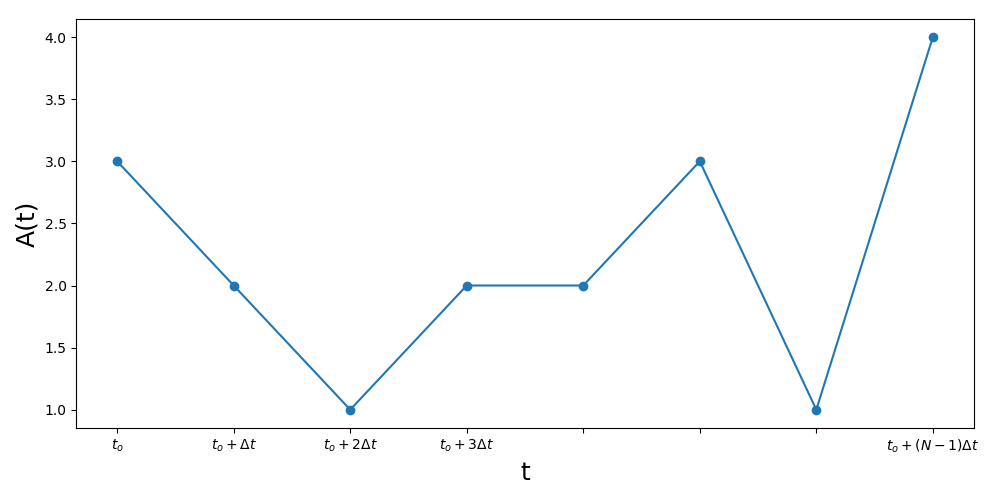
\includegraphics[width=0.9\textwidth]{discrete1}
	\end{figure}
\end{itemize}
\end{frame}
%------------------------------------------------
\begin{frame}{Discrete Time (or Space) Series}

\begin{figure}
		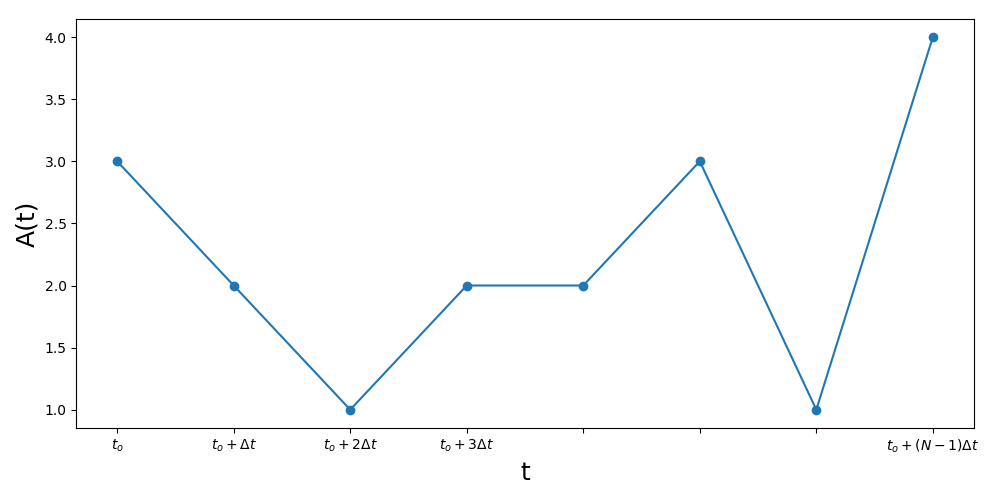
\includegraphics[width=0.9\textwidth]{discrete1}
	\end{figure}
	
\begin{itemize}
	\item $N$ $\rightarrow$ total number of data points
	\item $t_o+k\Delta t$ $\rightarrow$ $k^{th}$ data point ($0\leq k \leq N-1$)
	\item $A(t_k) = A(k) = A_k$ $\rightarrow$ notation for sampled series
	\item $T = N\Delta t$ $\rightarrow$ total period of sampling
\end{itemize}
\end{frame}

%------------------------------------------------
\subsection{Taylor's Frozen Turbulence Hypothesis} %
%------------------------------------------------
\begin{frame}{Taylor's Frozen Turbulence Hypothesis}

\begin{fancyquotes}
		If the velocity of the air stream which carries the eddies is very much greater than the turbulent velocity, one may assume that the sequence of changes in $u$ at the fixed point are simply due to the passage of an unchanging pattern of turbulent motion over the point, i.e. one may assume that
		$$u = \phi(t) = \phi\left(\frac{x}{U}\right)$$
		where $x$ is measured at time $t=0$ from the fixed point where $u$ is measured.
	\end{fancyquotes}
\end{frame}

%------------------------------------------------

\begin{frame}{Taylor's Frozen Turbulence Hypothesis}

\begin{itemize}
	\item As a result turbulence measurements that are made as a function of time can be translated into a corresponding spatial measurement.
	\item  This hypothesis is useful for cases where turbulent eddies evolve with a timescale longer than the time scale it takes the eddy to be advected past the sensor.
\end{itemize}
\end{frame}

%------------------------------------------------
\begin{frame}{Taylor's Frozen Turbulence Hypothesis}

\begin{itemize}
	\item Following Stull (1988), the substantial derivative is zero for Taylor's Hypothesis
	\item Thus, $$\frac{\partial \zeta}{\partial t} = -\overline{u}\frac{\partial \zeta}{\partial x}-\overline{v}\frac{\partial \zeta}{\partial y}-\overline{w}\frac{\partial \zeta}{\partial z}$$
	\item If we assume that $\overline{w}=0$ and write $U = \sqrt{\overline{u}^2 + \overline{v}^2}$, then
	$$\frac{\partial \zeta}{\partial t} = -U\frac{\partial \zeta}{\partial x_d}$$
	where $x_d$ indicates along the direction of the wind.
\end{itemize}
\end{frame}
%------------------------------------------------
\begin{frame}{Taylor's Frozen Turbulence Hypothesis}

\begin{itemize}
	\item We can also write Taylor's hypothesis in terms of wavenumber $k$ and frequency $f$:
	$$k = \frac{f}{U}$$
	where $k = 2\pi/\lambda$ and $f=2\pi/T$ for wavelength $\lambda$ and wave period $T$.
	\item $k$ has dimensions of radians per unit length.
	\item $f$ has dimensions of radians per unit time.
\end{itemize}
\end{frame}
%------------------------------------------------
\subsection{Estimating Dissipation Rate} %
%------------------------------------------------
\begin{frame}{Estimating Dissipation Rate}

\begin{itemize}
	\item Recall when we derived the turbulence kinetic energy balance equation that dissipation was written as:
	$$\epsilon = \nu \overline{\frac{\partial u_i^\prime}{\partial x_j}\frac{\partial u_i^\prime}{\partial x_j}}$$
	\item Assuming homogeneous isotropic turbulence, dissipation may be estimated as:
	$$\epsilon = 15\nu \overline{\left(\frac{\partial u^\prime}{\partial x}\right)^2}$$
	\item We can invoke Taylor's frozen turbulence hypothesis to rewrite as
	$$\epsilon = 15\nu \overline{\left(-\frac{1}{U}\frac{\partial u^\prime}{\partial t}\right)^2}$$
	where $\partial u^\prime/\partial t$ is approximated, for example, from measurements.
\end{itemize}
\end{frame}

%------------------------------------------------
\begin{frame}{Estimating Dissipation Rate}
$$\epsilon = 15\nu \overline{\left(-\frac{1}{U}\frac{\partial u^\prime}{\partial t}\right)^2}$$
\begin{itemize}
	\item Remember that dissipation occurs at very small time and space scales.
	\item Thus, our measurement probes must be small and sample at high frequencies.
	\item Examples are sonic anemometers or hot-wire probes.
\end{itemize}
\end{frame}

%------------------------------------------------
\subsection{Autocorrelation} %
%------------------------------------------------
\begin{frame}{Autocorrelation}

\begin{itemize}
	\item Consider the discrete autocorrelation, which measures the persistence of a wave within the duration of a discrete series.
	\item Existence of persistent features may point to particular physical phenomena (e.g., eddy).
	$$R_{AA} (L) = \frac{\displaystyle \sum\limits_{k=0}^{N-j-1} \left[ \left(A_k - \overline{A}_k\right)\left(A_{k+j}-\overline{A}_{k+j}\right)\right]} {\left[\displaystyle \sum\limits_{k=0}^{N-j-1} \left(A_k - \overline{A}_k \right)^2\right]^{1/2} \left[\displaystyle \sum\limits_{k=0}^{N-j-1} \left(A_{k+j} - \overline{A}_{k+j} \right)^2\right]^{1/2}}$$
	where the lag $L=j\Delta t$
\end{itemize}
\end{frame}
%------------------------------------------------
\begin{frame}{Autocorrelation}

\begin{itemize}
	\item Note that we use two different means depending on where we are in the time series
	$$\overline{A}_k = \frac{1}{N-j}\displaystyle \sum\limits_{k=0}^{N-j-1} A_k \qquad \overline{A}_{k+j} = \frac{1}{N-j}\displaystyle \sum\limits_{k=0}^{N-j-1} A_{k+j}$$
	\item If we assume that the data is stationary (homogeneous in space):
	$$R_{AA}(L) \simeq \frac{\overline{A_k^\prime A_{k+j}^\prime}}{\sigma_A^2}$$
	\item As lag increases, we use less of the series and so the statistical significance of $R_{AA}$ decreases.
	\item Thus, we compute $R_{AA}$ for the range of lags ($j=0$ to $j=N/2$). 
\end{itemize}
\end{frame}
%------------------------------------------------
\begin{frame}{Autocorrelation}
\begin{figure}
	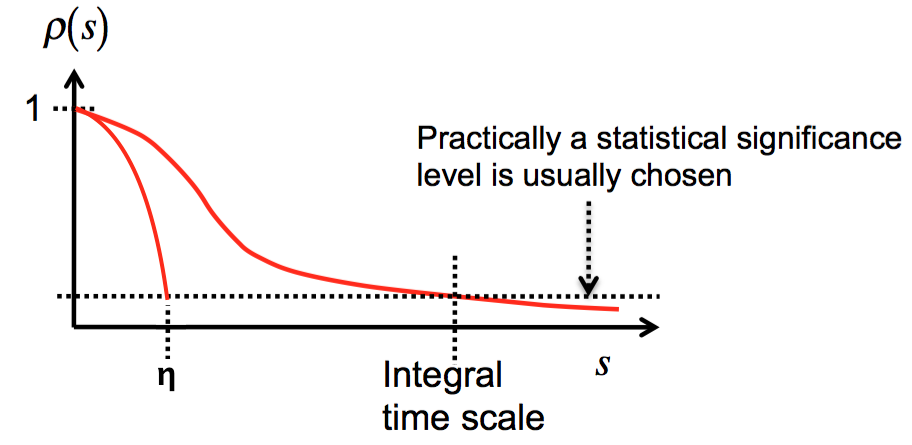
\includegraphics[width=0.65\textwidth]{auto1}
\end{figure}
\begin{itemize}
	\item Autocorrelation can aid in showing the persistence of an eddy
	\item Integral scale $\ell_o = \int_0^\infty R_{AA}(L)dL$ is a measure of the area over which a signal is correlated with itself (indicates largest eddies in the flow).
	\item Kolmogorov microscale is found by fitting a parabola to the near-origin points (see Tennekes and Lumley) and locating the x-intercept. This measures the smallest eddies that are dynamically significant in the flow.
\end{itemize}
\end{frame}

%------------------------------------------------
\subsection{Discrete Fourier Transform Review} %
%------------------------------------------------
\begin{frame}{Discrete Fourier Transform}
There are several ways to describe the frequency of our series.
\begin{itemize}
	\item $n$ = number of cycles per time period (from 1 to $N-1$)
	\item $\tilde{n}$ = cycles per second: $n/T = n/(N\Delta t)$
	\item $f$ = radians per second: $2\pi n /T = 2\pi n / (N\Delta t)$ 
\end{itemize}
~\\
Frequency values mean different things
\begin{itemize}
	\item $n=0 \rightarrow$ mean value
	\item $n=1 \rightarrow$ fundamental frequency (one wave fills $T$)
	\item $n>1 \rightarrow$ harmonics of the fundamental frequency
\end{itemize}
\end{frame}
%------------------------------------------------
\begin{frame}{Discrete Fourier Transform}

\begin{itemize}
	\item We can represent our series as the superposition of sine and cosine waves via Euler's formula [$\exp(ix) = \cos(x) + i \sin(x)$]
	$$A_k = \displaystyle \sum\limits_{k=0}^{N-1} F_A(n) e^{i2\pi n k / N}$$
	where $F_A(n)$ is the \textbf{discrete Fourier transform}.
	\item $F_A(n)$ is a complex number where the real part is the amplitude of the cosine waves and the imaginary part is the amplitude of the sine waves.
	\item $F_A(n)$ is a function of frequency because waves of different frequencies have to be multiplied by different amplitudes to reconstruct the signal.
\end{itemize}
\end{frame}
%------------------------------------------------
\begin{frame}{Discrete Fourier Transform}
\begin{itemize}
	\item If we have the discrete series, we can solve for the Fourier coefficients
	$$F_A(n) = \displaystyle \sum\limits_{k=0}^{N-1} \left(\frac{A_k}{N}\right)e^{-i2\pi n k / N}$$
	\item This is the forward transform, which converts from physical to phase space.
	\item Another name for this expression is \textbf{Fourier decomposition}.
\end{itemize}
\end{frame}

%------------------------------------------------
\subsection{Discrete Energy Spectrum} %
%------------------------------------------------
\begin{frame}{Discrete Energy Spectrum}
\begin{itemize}
	\item We are interested in how much variance of a discrete series is associated with a particular frequency.
	\item We are not interested in the phase of the waves
	\item In fact, we expect that a turbulent signal does not behave physically like a wave at all.
	\item It is still useful to break the turbulent signal into components of different frequencies, which we associate with eddies of different sizes.
	\item i.e., large eddies have low frequency and small eddies have high frequency
\end{itemize}
\end{frame}

%------------------------------------------------
\begin{frame}{Discrete Energy Spectrum}
\begin{itemize}
	\item Note that the signal power (power at different frequencies) is defined as:
	$$P = \frac{1}{T} \displaystyle \int A^2(t) dt$$
	\item So we need to find the square of the norm of our transform
	\begin{align*}
	F_A(n) &= \underbrace{F_r}_{\text{real}} + \underbrace{iF_i}_{\text{imag}}\\
	F_A^*(n) &= \underbrace{F_r - iF_i}_{\text{complex conjugate}}\\
	|F_A(n)|^2 &= F_A(n) F_A^*(n)\\
	&= (F_r+iF_i)(F_r - iF_i)\\
	&= F_r^2 -F_r iF_i + F_r iF_i +F_i^2\\
	&= F_r^2 + F_i^2
	\end{align*}
\end{itemize}
\end{frame}
%------------------------------------------------
\begin{frame}{Discrete Energy Spectrum}
\begin{itemize}
	\item In Matlab:
	$$|F_u(n)|^2 = \left[\frac{\text{fft}(u)}{\text{length}(u)}\right] .* \text{conj}\left[\frac{\text{fft}(u)}{\text{length}(u)}\right]$$
	\item If we sum up $|F_A(n)|^2$ from $n=1$ to $N-1$, we get the total biased variance
	$$\displaystyle \sum\limits_{n=1}^{N-1} |F_A(n)|^2 = \frac{1}{N}\displaystyle \sum\limits_{k=0}^{N-1} (A_k - \overline{A}_k)^2 = \sigma_A^2$$
	\item Thus, we say that the $|F_A(n)|^2$ is the portion of variance explained by waves of frequency $n$.
	\item Note: we don't sum over $n=0$ because that represents the mean value of the signal, which does not contribute to the variation of the signal about the mean.
\end{itemize}
\end{frame}
%------------------------------------------------
\begin{frame}{Discrete Energy Spectrum}
\begin{itemize}
	\item If we define $G_A(n) = |F_A(n)|^2$, then:
	$$\frac{G_A(n)}{\sigma_A^2}$$
	describes the fraction of the variance explained by frequency $n$. In this sense, it is analogous to the correlation coefficient.
	\item We can write the \textbf{discrete spectral energy} $E_A(n)$ as:
	$$E_A(n) = 2|F_A(n)|^2$$
	for $n=1$ to $n_f$ when $N$ is odd, or
	$$E_A(n) = 2|F_A(n)|^2$$ for $n=1$ to $n_f-1$ and 
	$$E_A(n) = |F_A(n)|^2$$ at $n=n_f$ when $N$ is even.
\end{itemize}
\end{frame}
%------------------------------------------------
\begin{frame}{Discrete Energy Spectrum}
\begin{itemize}
	\item The discrete spectral energy may be used for variables such as temperature, humidity, and velocity in order to separate the total variance into contributions by different frequencies.
	\item Be careful not to assume that spectra of temperature and humidity relate to eddy motions since variations of these variables can persist in a non-turbulent flow as a ``footprint'' of previous turbulent activity.
	\item An example is the residual layer that persists after sundown, when the gradients of moisture and temperature can maintain their shapes that were created during the convective boundary layer.
	\item The variance of velocity fluctuations $u^\prime$ has the same units as turbulence kinetic energy per unit mass - thus, the spectrum of velocity is often called the \textbf{energy spectrum}.
\end{itemize}
\end{frame}
%------------------------------------------------
\subsection{Spectral Density} %
%------------------------------------------------
\begin{frame}{Spectral Density}
\begin{itemize}
	\item Several theories use continuous spectra instead of discrete spectra.
	\item Instead of summing discrete spectra over all $n$ to obtain the total variance, they assume the existence of a \textbf{spectral energy density}, that can be integrated over $n$ to yield the total variance:
	$$\sigma_A^2 = \displaystyle \int_n S_A(n) dn$$
	\item The spectral energy density $S_A(n)$ has units of $A^2$ per unit frequency.
	\item We can approximate the spectral energy density as:
	$$S_A(n) = \frac{E_A(n)}{\Delta n}$$
\end{itemize}
\end{frame}
%------------------------------------------------
\begin{frame}{Spectral Density}
$$S_A(n) = \frac{E_A(n)}{\Delta n}$$
\begin{itemize}
	\item $\Delta n$ is the difference between neighboring frequencies.
	\item When $n$ is used to represent frequency, then $\Delta n = 1$. Other representations, such as $f$, do not necessarily lead to $\Delta n = 1$.
	\item The $S_A(n)$ points are plotted as curve to represent the spectrum.
	\begin{figure}
	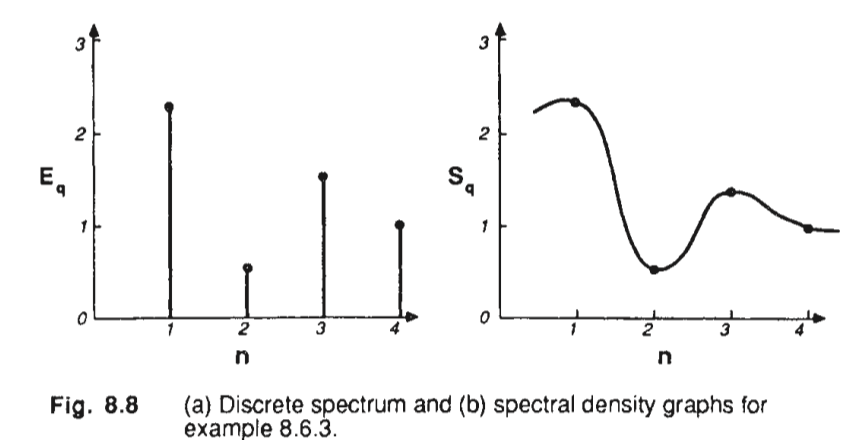
\includegraphics[width=0.65\textwidth]{spectra1.png}	
	\end{figure}
	\centering\tiny via Stull (1988)
\end{itemize}
\end{frame}
%------------------------------------------------
\begin{frame}{Spectral Density}

	\begin{figure}
	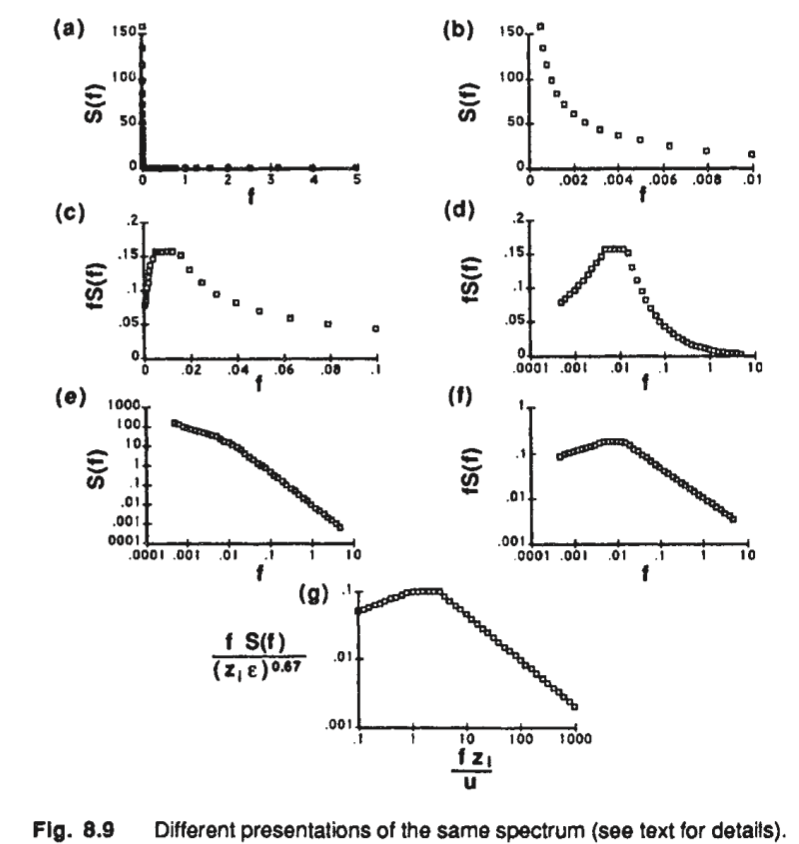
\includegraphics[width=0.65\textwidth]{spectra2.png}	
	\end{figure}
	\centering\tiny via Stull (1988)
\end{frame}
%------------------------------------------------
\begin{frame}{Spectral Density}
\textbf{linear-linear plots}
\begin{itemize}
	\item As in panel (a), area under curve between pair of frequencies is proportional to the portion of variance explained by that range of frequencies.
	\item Visually useless because high-frequency scales are masked by the large values at low frequencies.
	\item Alternative are to expand the low-frequency part of the spectrum (panel b), or to multiply the spectral density by $f$ (panel c).
	\item These approaches still focus on the spectral peak and lose information at high frequencies.
\end{itemize}
\end{frame}
%------------------------------------------------
\begin{frame}{Spectral Density}
\textbf{semi-log plots}
\begin{itemize}
	\item In this approach (panel d), $f \cdot S_A(f)$ is plotted against $\log(f)$
	\item Making the $x$-axis a log scale results in the expansion of the low-frequency parts of the spectrum.
	\item Multiplying the spectral density by $f$ results in the expansion of the high-frequency parts of the spectrum alongt he $y$-axis.
	\item The area under any part of the curve is proportional to the variance.
\end{itemize}
\end{frame}
%------------------------------------------------
\begin{frame}{Spectral Density}
\textbf{log-log plots}
\begin{itemize}
	\item This presentation (panel e) is $\log{S_A(f)}$ vs. $\log{f}$.
	\item A wide range of frequencies and spectral densities are discernible.
	\item Power laws (such as Kolmogorov's $-5/3$ law) appear as straight lines.
	\item The area under a curve is no longer proportional to variance.
\end{itemize}
\end{frame}
%------------------------------------------------
\begin{frame}{Spectral Density}
\textbf{log-log plots}
\begin{itemize}
	\item Another version of the log-log plot (panel f) is $\log{f \cdot S_A(f)}$ vs. $\log{f}$.
	\item Same characteristics of previous log-log plot.
	\item $f \cdot S_A(f)$ has the same units as variance, which makes normalization easier.
	\item The area under a curve is also no longer proportional to variance. 
	\item One last approach is a normalize (make dimensionless) the $x$-axis and $y$-axis by way of scaling variables (panel g).
\end{itemize}
\end{frame}


%------------------------------------------------
\subsection{Two-variable Spectra} %
%------------------------------------------------
\begin{frame}{Cross Spectra}
\begin{itemize}
	\item Using the ideas before for one variable, consider the cross spectra of two variables
	\begin{align*}
	G_{AB} &= F^*_A(n) F_B(n)\\
	&= (F_{Ar}-iF_{Ai})(F_{Br} + iF_{Bi})\\
	&= F_{Ar} F_{Br} - iF_{Ai} F_{Br} + F_{Ar} iF_{Bi} +F_{Ai}F_{Bi}\\
	&= C_o - iQ	
	\end{align*}
where the real parts make up the co-spectrum ($C_o$) and the imaginary parts make up the quadrative ($Q$) spectrum

\begin{align*}
C_o &= 	F_{Ar} F_{Br} + F_{Ai}F_{Bi}\\
Q &= F_{Ai} F_{Br} - F_{AR}F_{Bi}
\end{align*}
\end{itemize}
\end{frame}
%------------------------------------------------
\begin{frame}{Cospectrum}
\begin{itemize}
	\item Like with variance and energy spectrum, the sum over all frequencies of all co-spectral amplitudes is the covariance of $A$ and $B$.
	$$\displaystyle \sum\limits_{n=0}^{N-1} C_o(n) = \overline{A^\prime B^\prime}$$
	\item This is \textbf{not} the same as the spectrum of the time series of $A^\prime B^\prime$
	\item As a result, the co-spectrum can have negative values.
	\item Recall, energy spectrum cannot (magnitude).
\end{itemize}
\end{frame}
%------------------------------------------------
\begin{frame}{Discrete Energy Cospectrum}
\begin{itemize}
	\item We can write the \textbf{discrete cospectral energy} $E_A(n)$ as:
	$$E_{AB}(n) = 2|C_o(n)|^2$$
	for $n=1$ to $n_f$ when $N$ is odd, or
	$$E_{AB}(n) = 2|C_o(n)|^2$$ for $n=1$ to $n_f-1$ and 
	$$E_{AB}(n) = |C_o(n)|^2$$ at $n=n_f$ when $N$ is even.
\end{itemize}
\end{frame}
%------------------------------------------------
\begin{frame}{Cospectral Density}
\begin{itemize}
	\item We can approximate the co-spectral energy density as:
	$$CS_{AB}(n) = \frac{E_{AB}(n)}{\Delta n}$$
	\item And 
	$$\overline{A^\prime B^\prime} = \displaystyle \int_n CS_{AB}(n) dn$$
	\item As $CS_{AB}(n) \rightarrow \infty$ at high frequency, we have an indicator of local isotropy.
\end{itemize}
\end{frame}
%------------------------------------------------
\begin{frame}{Phase Spectrum}
\begin{itemize}
	\item The phase spectrum $\Phi$ is defined as:
	$$\tan{\Phi}=\frac{Q}{C_o}$$
	\item This is interpreted as the phase difference between the two time series $A$ and $B$that yields the greatest correlation for any frequency.
	\item This helps understand the physical structure of the flow.
\end{itemize}
\end{frame}

%------------------------------------------------
\end{document}

